
\chapter{Algebra}
Engingeering Mathematics begins by reviewing foundational algebra. Many of the skills used in this chapter are foundational mathematical tools that you will need to keep using repeatedly both in this course and beyond. Refer to the course website $<$\texttt{blackboard.aut.ac.nz}$>$ for additional review material covering the basics of algebra.

%%%%%%%%%%%%%%%%%%%%%%%%%%%%%%%%%%%%%%%%%%%%%
\section{Introductory Algebra}
Some of the foundational algebraic properties will be covered here. This section is not comprehensive, and the student should refer to an introductory algebra book if some of these properties are not clear.
\section*{Expanding and Factorising}
Multiplying algebraic expressions is usually called \emph{expanding}
and the reverse process is called \emph{factorising}. We usually use the word factorising in New Zealand, however, most textbooks use the term factoring. We will use both terms interchangeably in this course. Factor(is)ing and expanding can be viewed as opposite operations; one undoes the other.  

\textbf{Example} Expand the following algebraic expression (remove the brackets): $x(x-7)$\\
\textbf{Solution} $x(x-7)=x^2-7x$

\textbf{Example} Expand: $(x+3)(x-3)$. Note there is a mnemonic \textbf{\sc{FOIL}} that may help you remember how to expand here: First, Inside, Outside, Last.\\
\textbf{Solution} $=x^2+3x-3x-9=x^2-9$\\

\textbf{Example} Expand: $x(x+1)(x-2)$\\
\textbf{Solution} Begin by expanding the first two terms:
\begin{align*} &=(x^2+1)(x-2)\\
&=x^3-2x^2+x-2
\end{align*}

Factoring involves removing common terms from expressions and then writing them as products. Recall that product means multiply and can be shown algebraically by writing terms in brackets. 

\textbf{Example} Factor the following algebraic expression: $2x-4x^2+6x^3$\\
\textbf{Solution} Remove a common factor of $2x$: $\,2x-4x^2+6x^3=2x(1-2x^2+3x^3)$

\textbf{Example}
Factorise: $x^{2} -5 x -6$. Note that this is a quadratic equation and will factor into two sets of brackets.\\
\textbf{Solution} For these examples you are required to find a pair of numbers that add together to give $ -5$ and multiply together to give $ -6$. In this case the numbers are $ -6$ and $ +1$. So the answer is
\begin{equation*}x^{2} -5 x -6 =\left (x -6\right ) \left (x +1\right )
\end{equation*}

This can easily be verified by expanding the brackets.\\

\textbf{Example} Factor: $x^2-4x+4$\\
\textbf{Solution} $=(x-2)(x-2)=(x-2)^2$

%%%%%%%%%%%%%%%%%%%%%%%%%%%%%%%%%%%%%%%%%%%%% 
\section*{Solving Equations}
An equation is a mathematical expression separated by two lines of \textit{equal} length ($=$). There must be symbols (either numbers or algebraic letters) on both sides of the equality. For example, $5x=25$ is an equation, however, $5(1)+25$ is just an expression. An equation can be solved; in the previous example, $x=5$ is a solution, whereas an expression may be simplified ($5(1)+25=30$). Conversely, factoring the quadratic $x^2-4x+4=(x-2)^2$ is \textit{not} solving the expression.

When solving an equation the order of operations is important. The acronym \textbf{BEDMAS} is used for simplifying expressions starting with B=brackets, and ending with S=subtraction. The reverse is true for solving equations. First you must undo any subtraction or addition to isolate the variable.

\textbf{Example} Solve the equation for $x$: $x-11=7$\\
\textbf{Solution} To isolate $x$ we will add 11 to both sides: $x-11\textbf{+11}=7\textbf{+11}$\\
And simplify: $x=18$

\textbf{Example} Solve the equation: $2x+5=10$\\
\textbf{Solution} To isolate $x$ first we have to subtract 5 from both sides: $2x=10-5$\\
And then we divide both sides by 2: $\frac{2x}{2}=\frac{10-5}{2}$\\
And simplify: $x=\frac{5}{2}$

\begin{tcolorbox}
A general rule for solving equations is that you can do any mathematical operation to the equation as long as you do it to both sides. For example, add 5 to both sides, divide both sides by 2, multiply both side by $\sin(x)$, and so on.
\end{tcolorbox}

\textbf{Example} Find $x$: $x^2+1=3$\\
\textbf{Solution} Subtract 1 from both sides: $x^2=2$\\
Recall BEDMAS in reverse order, now we have an exponent. To solve for a power of 2, take the square root of both sides: $\sqrt{x^2}=\sqrt{2}$, and simplify to $x=\sqrt{2}$

%%%%%%%%%%%%%%%%%%%%%%%%%%%%%%%%%%%%%%%%%%%%%
\section*{Indices}
Indices go by a few different names, sometimes they are called powers or exponents. In the expression $x^3$ the index, exponent, or power is $3$. This does not have to be an integer, or even a number: $x^n$ has index $n$; $x^{\frac{2}{3}}$ has a fractional exponent; $x^{-1}$ has a negative exponent; and $x^{\cos x}$ has another expression for its power.

\subsection*{The Rules of Exponents}
\begin{tcolorbox}
	\begin{itemize}
		\item $x^n$: $x$ is called the base and $n$ the exponent (or power)
		\item When multiply exponents of the same base, add the exponents: $x^3\times x^4=x^{3+4}=x^7$
		\item When dividing exponents of the same base, subtract the exponents:
		$\frac{x^6}{x^5}=x^{6-5}=x^1$
		\item If an expression is raised to \textit{another} power, multiply the exponents:
		$x^{3^4}=x^{3\times 4}=x^{12}$
	\end{itemize}
\end{tcolorbox}	

\subsection*{Negative Exponents}
One of the most important rules for manipulating mathematics is the exponent of negative one. A negative power is equivalent to the inverse of the same expression with a positive power. (Inverse means one divided by the same expression.)\\

\begin{tcolorbox}
	\hspace{1cm}$x^{-1}=\frac{1}{x}$ \hspace{2cm}$x^{-4}=\frac{1}{x^4}$\hspace{2cm}$\frac{2}{7y^3}=\frac{2y^{-3}}{7} $\hspace{2cm}$2^{-3}=\frac{1}{2^3}=\frac{1}{8} $
\end{tcolorbox}	

\subsection*{Fractional Exponents}
Exponents can decimal numbers, integers, expressions, variables, and also fractions. Fractional exponents can written using a root sign, this is called surd form. $x^{\frac{1}{2}}$ is also known as the square root of $x$. Using rules of exponents you can see that $x^{\frac{1}{2}}\times x^{\frac{1}{2}}=x^{\frac{1}{2}+\frac{1}{2}}=x^1=x$. Converting between surd and index form is quite handy, especially when we get to differentiation using the power rule.
\begin{tcolorbox}\begin{alignat*}{5}
\textrm{Index form: }\qquad&x^{\frac{1}{2}}&\qquad\qquad x^{\frac{3}{4}} &\qquad\qquad 64^{\frac{1}{3}}&\qquad\qquad x^\frac{a}{b}\\
\textrm{Surd form: }\qquad&\sqrt{x}&\qquad \sqrt[4]{x^3}&\qquad\qquad\sqrt[3]{64}&\qquad \sqrt[b]{x^a}
\end{alignat*}\end{tcolorbox}
	
%%%%%%%%%%%%%%%%%%%%%%%%%%%%%%%%%%%%%%%%%%%%%
\section{Functions}	
A function is a mathematical relationship between groups. Given an element in one group, the function says how to get to the other group. For example the function could be a formula that says if you have $x$, the output is $2x$. This can be written as $f(x)=2x$ where $f(x)$ is called function notation and in Cartesian coordinates also means $y=f(x)$. We can depict this function visually using $x$ and $y$ coordinates. Begin by selecting some inputs ($x$ values) and then calculate the outputs ($f(x)$ values) from the formula $f(x)=2x$.

This method is called making a table of values and in this example any real number for $x$ produces exactly one output for $y$ (also a real number). The figure below plots the points on an $(x,y)$ grid. Connecting the points creates the line $y=2x$.
\clearpage
\begin{multicols}{2}
\begin{center}
\begin{tabular}{clr}  
	\toprule
	inputs&outputs&\\
$x$&$f(x)=2x$& \\
	\midrule
	$-2$    & $f(-2)=2(-2)$&$=-4$\\
	\midrule
$-1$ & $f(-1)=2(-1)$&$=-2$ \\
\midrule
$0$ & $f(0)=2(0)$&$=0$ \\
\midrule
$1$ & $f(1)=2(1)$&$=2$ \\
\midrule
$2$ & $f(2)=2(2)$&$=4$ \\
	\bottomrule
\end{tabular}
\captionof*{tabular}{A \textbf{table of values} for the function $f(x)=2x$}
\end{center}
\columnbreak
\begin{center}
\begin{tikzpicture}
\begin{axis}[
scale=1.1,
axis lines=center,
ymax=4,ymin=-4,
xmax=4,xmin=-4,
xlabel=$x$,ylabel=$y$,
]
\addplot [<->,dashed,domain=-2:2,thick, samples=100, black] {2*x};
\node[anchor=south] at (axis cs:1.8,0.5) {$f(x)=2x$};
\addplot[mark=*] coordinates {(-2,-4)};
\addplot[mark=*] coordinates {(-1,-2)};
\addplot[mark=*] coordinates {(0,0)};
\addplot[mark=*] coordinates {(1,2)};
\addplot[mark=*] coordinates {(2,4)};
\end{axis}
\end{tikzpicture}
\captionof*{tikzpicture}{A \textbf{plot of the points} showing a linear relationship}
\end{center}
\end{multicols}

Lets write a precise definition of a function:
\begin{tcolorbox}
	A function $f(x)$ has exactly one output value, $y$, for any given input value, $x$.
\end{tcolorbox}
In the line plotted above, we see that every $x$ value has only one corresponding $y$ value. This means that $y=2x$ is a function. Conversely, a relationship that has two or more output values is \textbf{not} a function. \\ 
\begin{multicols}{2}
	\begin{center}
\resizebox{0.5\textwidth}{0.5\textwidth}{%
	\begin{tikzpicture}
	\begin{axis}[
	scale=1.1,
	axis lines=center,%width=4cm,height=4cm,
	ymax=3,ymin=-3,
	xmax=3,xmin=-3,
	xlabel=$x$,ylabel=$y$,%	ytick=\empty,	
	]
	\addplot [domain=-180:180, samples=100] ({2*cos(x)},{2*sin(x)});
	\addplot[mark=*] coordinates {(1,1.732)};
	\addplot[mark=*] coordinates {(1,-1.732)};
	\addplot [mark=none,dashed] coordinates {(1, -3) (1, 3)};
	\end{axis}
	\end{tikzpicture}
}	\end{center}
\columnbreak
The circle has two output values at $x=1$: both $y=+\sqrt{3}$ and $y=-\sqrt{3}$ are points on the circle.

The dashed line in the figure represents what is called the \textit{verical line test}. If a vertical line passes through more than one point on a curve, then it is not considered a function.

\subsection*{Domain \& Range}
The domain of a function is the set of all inputs that are valid; usually these are the $x-$values. The range of a function is the set of all outputs that are valid; usually these are the $y-$values. For the line we plotted above, $f(x)=2x$, any value could be substituted into the function, therefore the domain was all the real numbers. This is written as: Domain $x \in \mathbb{R}$. Similarly the range was all the $y-$values, or  $y \in \mathbb{R}$. We will return to domain and range later.
\end{multicols}

%%%%%%%%%%%%%%%%%%%%%%%%%%%%%%%%%%%%%%%%%%%%%
\section*{Linear Functions}
Linear functions can represented nicely as a straight line on a standard Cartesian ($x,y$) coordinate system. The following are all examples of linear functions, and not surprisingly, can be drawn as a lines.

%linear function examples here
\begin{figure}[H]
	\begin{subfigure}[b]{0.33\textwidth}
		\centering
		\resizebox{\linewidth}{!}{
			\begin{tikzpicture}
			\draw[<->] (-3,0) -- (3,0) node[right] {$x$};
			\draw[<->] (0,-3) -- (0,3) node[above] {$y$};
			\draw[ultra thick,<->, scale=1,domain=-3:3,smooth,variable=\x,black] plot ({\x},{2});		
			\end{tikzpicture}
			
		}  \caption{zero slope}
	\end{subfigure}
	\begin{subfigure}[b]{0.33\textwidth}
		\centering
		\resizebox{\linewidth}{!}{
			\begin{tikzpicture}
		\draw[<->] (-3,0) -- (3,0) node[right] {$x$};
		\draw[<->] (0,-3) -- (0,3) node[above] {$y$};
		\draw[dashed,thick,->] (-2,-1) -- (-2,2) node[xshift=-0.4cm, yshift=-1cm] {rise};
		\draw[dashed,thick,->] (-2,2) -- (1,2) node[xshift=-1cm,above left] {run};
			\draw[ultra thick,<->,scale=1,domain=-3:2.3,smooth,variable=\x,black] plot ({\x},{\x+1});
			\end{tikzpicture}
		}  \caption{positive slope}
	\end{subfigure}
	\begin{subfigure}[b]{0.33\textwidth}
		\centering
		\resizebox{\linewidth}{!}{
			\begin{tikzpicture}
			\draw[<->] (-3,0) -- (3,0) node[right] {$x$};
		\draw[<->] (0,-3) -- (0,3) node[above] {$y$};
		\draw[ultra thick,<->,scale=1,domain=-3:3,smooth,variable=\x,black] plot ({\x},{-0.25*\x-0.5});
			\end{tikzpicture}			
		}  \caption{negative slope}
	\end{subfigure}
\end{figure}

Linear functions have a few characteristics that we will get used to manipulating. The slope of a line is often represented by the letter $m$ and can be calculated by taking any two points on the line $(x_1,y_1)$, and $(x_2,y_2)$ and using the formula: $m =\frac{y_{2} -y_{1}}{x_{2} -x_{1}}$. This is also known as the \textit{gradient}, a term that will be used often in calculus.


\begin{tcolorbox}
	\begin{center}
	slope$=$m$=$gradient$=\frac{rise}{run}=\frac{\Delta y}{\Delta x}=\frac{y_{2} -y_{1}}{x_{2} -x_{1}}$
\end{center}\end{tcolorbox}	

 
 The standard form for an equation of a line is: $y =m x +c$ where $m$ is the slope described above, and $c$ is the $y-$intercept. Alternatively if you know the slope and any given point $(x_1,y_1)$, the equation of a line is $y -y_{1} =m (x -x_{1})$ where $x_1$ and $y_1$ are the coordinates of a point on the line.

Note that a vertical line has an \textit{undefined} slope. Using the formula above, a vertical line has a slope of $m=\frac{\Delta y}{0}$ because it has the same $x$ values everywhere. Dividing by zero is undefined (try on your calculator) and therefore a vertical line is not considered a function.

\textbf{Question} Does a vertical line pass or fail the vertical line test? Why?\\

%%%%%%%%%%%%%%%%%%%%%%%%%%%%%%%%%%%%%%%%%%%%%
\section*{Quadratic Functions}
 A quadratic relationship scales with the square of the input values. The following are all examples of quadratic functions:
 \begin{itemize}
 	\item $ y=x^2-5$
 	\item $ s(t)=-4.9t^2-15t+3$
 	\item $ b^2+7b-1=0$
 \end{itemize}
Note that they all have a power of 2 in the equation, and that is the highest exponent. This type of relationship is also referred to as parabolic. When a parabola equation is plotted, the solutions represent where the function crosses the $x-$axis. These points are called roots.
 
 \textbf{Example} Find the roots of the following parabolas.
 %linear function examples here
 \begin{figure}[H]
 	\begin{subfigure}[b]{0.33\textwidth}
 		\centering
 		\resizebox{\linewidth}{!}{
 			\begin{tikzpicture}\begin{axis}[
 			axis lines=center,
 			ymax=3,ymin=-1,
 			xmax=3,xmin=-3,
 			xlabel=$x$,ylabel=$y$,
 			ytick=\empty,xtick=\empty,
 			]
 			\addplot [<->,domain=-1.7:1.7,thick, samples=200, black] {x^2};
 			\end{axis}		
 			\end{tikzpicture}
 		}  \caption{$y=x^2$}
 	\end{subfigure}
 	\begin{subfigure}[b]{0.33\textwidth}
 		\centering
 		\resizebox{\linewidth}{!}{
 			\begin{tikzpicture}
 			\begin{axis}[
 			axis lines=center,
 			ymax=3,ymin=-3,
 			xmax=3,xmin=-3,
 			xlabel=$x$,ylabel=$y$,
 			ytick=\empty,xtick=\empty,
 			]
 			\addplot [<->,domain=-3:3,thick, samples=200, black] {0.3*x^2-1};
 			\end{axis}	
 			\end{tikzpicture}
 		}  \caption{$y=0.3x^2-1$}
 	\end{subfigure}
 	\begin{subfigure}[b]{0.33\textwidth}
 		\centering
 		\resizebox{\linewidth}{!}{
 			\begin{tikzpicture}
 			\begin{axis}[
 			axis lines=center,
 			ymax=4.5,ymin=-3,
 			xmax=3,xmin=-4,
 			xlabel=$x$,ylabel=$y$,
 			ytick=\empty,xtick=\empty,
 			]	
 			\addplot [<->,domain=-3.5:1.5,thick, samples=200, black] {-x^2-2*x+3};
 			\end{axis}	
 			\end{tikzpicture}			
 		}  \caption{$f(x)=-x^2-2*x+3$}
 	\end{subfigure}
 \end{figure}
\textbf{Solution} The roots are where the function intersects the $x-$axis. The $x-$axis is where $y=0$, so we will substitute $y=0$ into the functions and solve the equations for $x$.\\
\textbf{(a)} Substituting in $y=0$ gives the equation $0=x^2$. This solves directly for $x=0$. Therefore the root to $y=x^2$ is $0$.\\
\begin{multicols}{2}
\textbf{(b)} Solve the equation 
\begin{align*}
0&=0.3x^2-1\\
1&=0.3x^2\\
\frac{1}{0.3}&=x^2\\
\sqrt{\frac{1}{0.3}}&=x\\
\textrm{Therefore }x&=\pm 1.826
\end{align*}\\
\columnbreak

\textbf{(c)}
\begin{align*}
0&=-x^2-2x+3\quad\textrm{here you can divide by }-1\\
0&=x^2+2x-3\quad\textrm{and factor}\\
0&=(x+3)(x-1)\\
&\textrm{Therefore }x=-3\textrm{ and }x=1
 \end{align*}
\end{multicols}
The parabola from part (c) above was solved by factoring. Not all quadratic equations can be solved in this manner. The standard form of a quadratic equation is written $a x^{2} +b x +c =0$. If we solve this equation for $x$ we get the quadratic formula:
 $$x =\frac{ -b \pm \sqrt{b^{2} -4 a c}}{2 a}$$ 
 where $a,b,$ and $c$ are coefficients ($a\ne0$). Note here there are two possible solutions because of the plus-minus sign ($\pm$).
%%%%%%%%%%%%%%%%%%%%%%%%%%%%%%%%%%%%%%%%%%%%%
\section{Polynomials}
 A polynomial is a type of function that comes up a lot. The quadratic equations above are all examples of polynomials. The standard form of a quadratic equation is shown below with some of the terminology.
 \begin{center}
 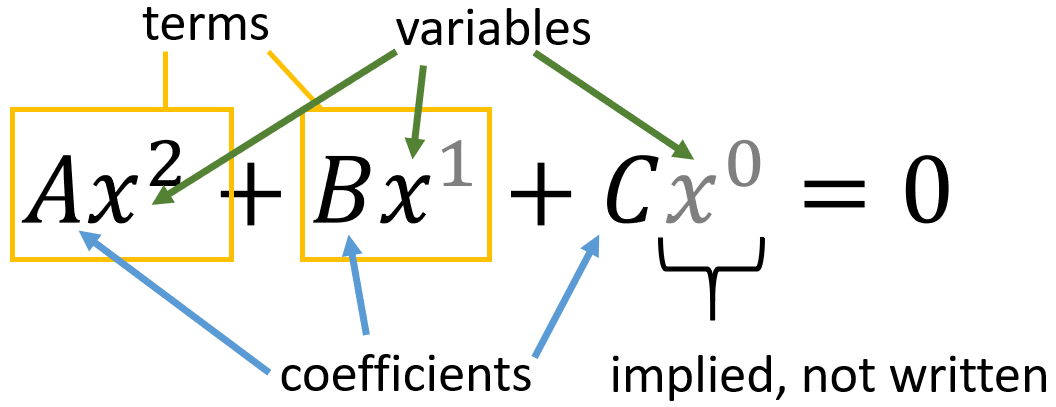
\includegraphics[width=0.6\textwidth]{poly}
\end{center}
The prefix \textit{poly} means many, and polynomials are not limited to three terms. The general form of a polynomial can be written as:
$$ A_1x^n+A_2x^{n-1}+A_3x^{n-2}+\dots+A_nx^1+C=0 $$
where the terms are written in decreasing powers of $x$, with
\vspace{-0.5cm}\begin{itemize}
	\setlength\itemsep{0em}
	\item $n\ge 0, n\in \mathbb{Z}$. This means the exponents must be integers.
	\item $A_1, \dots, A_n$ are real numbers.
	\item $C$ is a constant.
	\item The order or degree of the polynomial is $n$ (the highest exponent).
	\item Here, $x$ is the variable. You may have more than one variable in a polynomial, for example $4x^2+y-xy+4$ is a valid polynomial.
\end{itemize}
 
 
 %%%%%%%%%%%%%%%%%%%%%%%%%%%%%%%%%%%%%%%%%%%%
 \section{Systems of Equations}
 A system of equations means having more than one relationship represented within a common context. Revenue and costs may have different functions but both relate to the same product. We will study systems composed of two equations and two unknowns. Systems with more equations and more variables are possible and will be covered in future courses. Three approaches to solve systems of equations will be covered here:
 \begin{itemize}
 	\setlength\itemsep{0em}
 	\item graphing
 	\item elimination
 	\item substitution
 \end{itemize}
 
It helps if you can visualise the shape of the two functions so that the meaning of the solution is clear in your mind. Later in the course we will find the area between two curves using integration where the intersection of these two curves represents the solution to a system of two equations. See section XX.
 
 We know that linear equations in two variables are represented by straight lines. Straight
 lines will always intersect unless they are parallel. The coordinates of the point of intersection of the straight lines is called the solution. you could use a graphical method or one of the two algebraic methods (substitution or elimination) to find the solution.  We will start with a graphical method. 
 
 \textbf{Example} Find the solution to the set of linear relationships given by:
 $$2y=x-4$$
 $$y=\frac{x}{4}$$
  \begin{multicols}{2}
 \textbf{Solution} 
 	
 	Here we have two linear equations (we know they are linear because the highest exponent is 1) and if the lines intersect, that point of intersection represents a solution. 
 	
 	From the plot we can see the point of intersection is $(8,2)$. Therefore the solution to the system of linear equations is $(8,2)$. Try plotting the lines yourself at \url{www.desmos.com/calculator}.
 	\columnbreak
 \begin{center}
 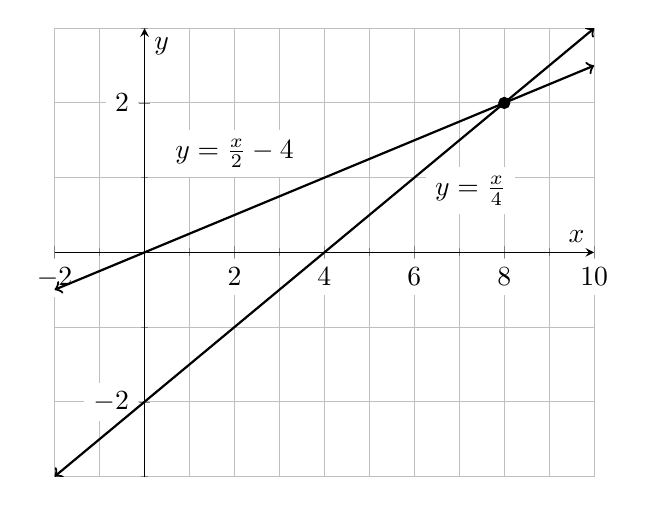
\begin{tikzpicture}
 \begin{axis}[
 grid=both,
 minor tick num=1,
 axis lines=center,
 xmax=10,xmin=-2,
 ymax=3,ymin=-3,
 xlabel=$x$,ylabel=$y$,
 ticklabel style={fill=white},
 ]	
 \node[anchor=south,fill=white] at (axis cs:2,1) {$y=\frac{x}{2}-4$};
 \node[anchor=south,fill=white] at (axis cs:7.25,0.5) {$y=\frac{x}{4}$};
 \addplot [<->,domain=-2:10,thick, samples=100, black] {0.5*x-2};
 \addplot [<->,domain=-2:10,thick, samples=100, black] {0.25*x};
 \addplot[mark=*] coordinates {(8,2)};
 \end{axis}	
 \end{tikzpicture}			
\end{center}
\end{multicols}
 
 Its not always convenient to graph a system of equations to find the solution; you may not have access to a computer, or the solution may not be integers. Solving by direct substitution is the next method.\\
 
 \textbf{Example} Consider the system of equations
 \begin{align}x^{2} +y^{2} &  = 25 \tag{1} \\
 3 y +x &  = 15 \tag{2}\end{align}
 \textbf{Solution} Without knowing what the functions look like or plotting them, we can isolate a variable and substitute it into the other equation. Rearrange equation (2) to isolate $x$ and substitute into equation (1):
$$x =  15 -3 y $$
 Equation (1) becomes
 \begin{align*}(15-3y)^2+y^2 &  =  25 \tag{expand and simplify}\\
 225-90y+9y^2+y^2&=25\\
 10 y^{2} -90 y +200 &  =  0 \tag{divide by 10}\\
 y^{2} -9 y +20 &  = 0 \tag{factor the quadratic}\\
 \left (y -5\right ) \left (y -4\right ) &  =  0 \\
 \text{Either }\quad y -5 &  =  0\quad\text{ so }\quad y =5 \\
 \text{or }\quad y -4 &  =  0\quad\text{ so }\quad y =4\end{align*}
 
Lastly, back-substitute the $y-$values into equation (2): 
 
 When $y =5$, $3 y +x =15 \leadsto 15 +x =15 \Longleftrightarrow x =0$. This means $\left (0 ,5\right )$ is a solution. 
 
 When $y =4$, $3 y +x =15 \leadsto 12 +x =15 \Longleftrightarrow x =3$. This means $\left (3 ,4\right )$ is a solution. 
 Note there are two solutions here. Verify by graphing the functions.
 
The third method is called elimination and works by eliminating one of the variables from the equation set, then solving for the other variable.

\textbf{Example} Solve the system by the method of elimination:


 \section*{Special Cases}
  \begin{multicols}{2}
  Consider the parallel lines shown. What is the solution to this system? Parallel lines will never meet by definition and so will have no point of intersection. In this case the system has no solution -- which is a perfectly valid solution!
  
  Sometimes the two equations will be two different representations of the same line. Imagine two line plotted on top of one another. In this case the system has an infinite number of solutions because every single point on the first function is also on the second function. 
 	\columnbreak
 	\begin{center}
 		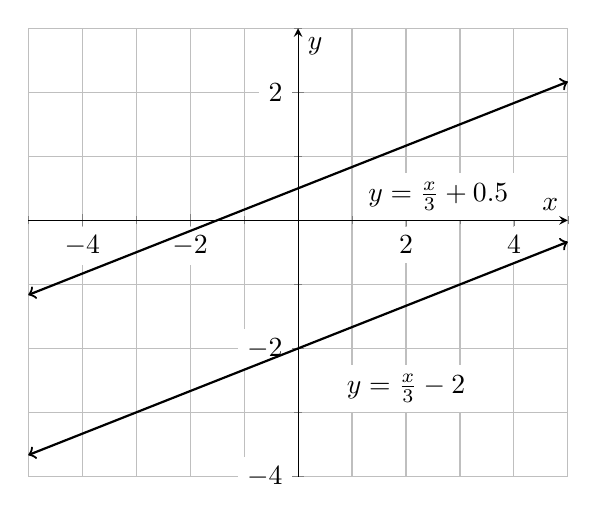
\begin{tikzpicture}
 		\begin{axis}[
 		grid=both,
 		minor tick num=1,
 		axis lines=center,
 		xmax=5,xmin=-5,
 		ymax=3,ymin=-4,
 		xlabel=$x$,ylabel=$y$,
 		ticklabel style={fill=white},
 		]	
 		\node[anchor=south,fill=white] at (axis cs:2,-3) {$y=\frac{x}{3}-2$};
 		\node[anchor=south,fill=white] at (axis cs:2.6,0) {$y=\frac{x}{3}+0.5$};
 		\addplot [<->,domain=-5:5,thick, samples=100, black] {0.333*x-2};
 		\addplot [<->,domain=-5:5,thick, samples=100, black] {0.333*x+0.5};
 		\end{axis}	
 		\end{tikzpicture}			
 	\end{center}
 \end{multicols}
 
 \textbf{Example}\\
 If you start with a linear equation such as $y -2 x =3$ and multiply each term by a constant you will get an equivalent equation. If you multiply the equation by another number you
 will get a further equivalent equation.
 \begin{equation*}y -2 x =3
 \end{equation*}
 
 Multiply by $2$
 \begin{equation*}2 y -4 x =6
 \end{equation*}
 
 Multiply by $ -3$
 \begin{align*} -3 y +6 x &  =   -9 \\
 \text{or }6 x -3 y +9 &  =  0\end{align*}
 
 We know these are both just different ways of writing the original equation $y -2 x =3$ or $y =2 x +3$. To say the system has an infinite number of solutions we are really saying every point
 on $y =2 x +3$ is a solution. 
 
 
 
 \section*{Guidelines for Solving Systems of Equations}
 These guideline provide a useful way to tackle any problems where equations are involved. 
 \begin{tcolorbox}
 	
  \begin{enumerate}\setlength\itemsep{0em}
 	\item Identify the variables. We often call them $x$ and $y$, but you may chose any name or letter you want. 	
 	\item Express all unknown quantities in terms of the variables. 	
 	\item Set up a system of equations using the facts provided by the problem.	
 	\item Solve the system of equations and use the solution to check it satisfies the conditions of the
 	problem. Write a sentence describing the answer to the original problem.  
 \end{enumerate}
\end{tcolorbox}
 
 \textbf{Example} It takes a boat travelling downstream 1 hour to cover the 20 mile distance. On the return trip it take the boat 2.5 hours. What is the speed of the boat and the speed of the current?\\
 \textbf{Solution} This is about a boat travelling with the current and against the current and depends on you knowing that velocities are vectors that can be added and subtracted. Let the speed of the boat be $x$ \mbox{mi}$/$\mbox{h} and the speed of the current be $y$ \mbox{mi}$/$\mbox{h}. 
 	\begin{align*}\text{Upstream speed} &  =  x -y \\
 	\text{Downstream speed} &  =  x +y\end{align*}
 	\begin{align}\text{Speed} &  =  \frac{\text{Total distance}}{\text{Total time}} \nonumber  \\
 	\text{so Total distance} &  =  \text{Speed} \times \text{Total time} \nonumber  \\
 	20 \textrm{ miles } &  =  \left (x +y\right ) \times 1 \textrm{ hour} \nonumber  \\
 	20 &=x +y \tag{1} \\
 	\text{Also}\quad 20 \textrm{ miles }&  =  \left (x -y\right ) \times \frac{5}{2} \textrm{ hours}\nonumber  \\
 	8 &=x -y \tag{2}\end{align}
 Now we can add equations (1) and (2) and $y$ is eliminated
 \begin{align*}28 &  =  2 x \\
 x &  =  14\end{align*} \\
 Back-substitute into either equations (1) or (2) to solve for $y$:
$$ y =  6$$
 \textbf{Check:} \\\relax The boat travels
 at 14 $\mbox{mi}$/$\mbox{h}$ and the current travels at 6 $\mbox{mi}$/$\mbox{h}$ so the effective speed of the
 boat is 20 $\mbox{mi}$/$\mbox{h}$. At 20 $\mbox{mi}$/$\mbox{h}$ the 20 $\mbox{mi}$ trip took $1$ $\mbox{h}$. Upstream the speed is 8 $\mbox{mi}$/$\mbox{h}$. \
 \begin{align*}\text{Total time} &  =  \frac{\text{Total distance}}{\text{Speed}} \\
 &  =  \frac{20}{8} =\frac{5}{2} \text{ h}\end{align*}
 
 Therefore the speed of the boat is 14 $\mbox{mi}$/$\mbox{h}$ and the speed of the current is 6 $\mbox{mi}$/$\mbox{h}$. 
 
 
 
 
 
%%%%%%%%%%%%%%%%%%%%%%%%%%%%%%%%%%%%%%%%%%%%%
\section{Exercises} 
 
\begin{enumerate}
	\item Remove the brackets 
	\begin{enumerate}
		\item $ -\left (x +y\right )$ 
		\item $ -3 (5 x -2 y)$ \end{enumerate}
	
	\item Evaluate $\left (\frac{1}{3} \div \frac{1}{6}\right ) +\frac{1}{2}$ 
	
	\item Calculate the value of 
	\begin{enumerate}
		\item $\left (15.3\right )^{0}$ 
		\item $10^{ -2}$ \end{enumerate}
	\item Simplify 
	\begin{enumerate}
		\item $\left (3 a^{2} b\right )^{2}$ 
		
		\item $\genfrac{(}{)}{}{}{x}{3}^{3} x^{3}$ \end{enumerate}
	
	
	\item Evaluate $\sqrt[{4}]{2.7}$ accurate to 2 decimal places. 
	
	\item Remove the brackets and simplify 
	
	
	\begin{enumerate}
		\item $\left (x^{2} +5 x -1\right ) -\left (2 x -3\right )$ 
		
		\item $\left (2 x -1\right ) \left (2 x +1\right )$ \end{enumerate}
	
	
	\item Factorise the expressions 
	\begin{enumerate}
		\item $x^{2} +11 x +28$ 	
		\item $2 x^{2} -5 x -12$ 
		\end{enumerate}
	\item Simplify $\frac{x^{2} +5 x +6}{x^{2} +2 x -3}$ by factorising and then cancelling 
	
	\item Solve the equations 
	
	
	\begin{enumerate}
		\item $7 x -16 =\frac{2}{3} x +4$ 
		
		\item $\left (x -2\right )^{2} =15$ \end{enumerate}

	\item Solve the equations 
	
	
	\begin{enumerate}
		\item $x^{2} -2 x -8 =0$ by factorising. 
		
		\item $2 x^{2} +5 x -4 =0$ by using the quadratic formula. \end{enumerate}
	
	
	\item
	Make $t$ the subject of the equation 
	
	
	\begin{enumerate}
		\item $v =u +a t$ 
		
		\item $l =l_{0} \left (1 +\alpha  t\right )$ \end{enumerate}
	
	
	\item 
	The volume of a pipe with length $l$, inner radius $r$ and outer radius $R$ is $V =\pi  \left (R^{2} -r^{2}\right ) l\text{.}$ Find the volume when $R =3.1 \mbox{m}$, $r =2.2 \mbox{m}$ and $l =5.3 \mbox{m}\text{.}$ 
	
	\item  Draw the graph of $y =x^{2} -3$ 
	
	\item  Find the distance between the points $\left (2 , -3\right )$ and $\left (5 , -1\right )\text{.}$ 
	
	\item  Find the $x$ and $y$ intercepts for the graph of $y =x^{2} -3.\vspace{+5.000000cm}$ 
	
	\item    
	\setlength\fboxrule{0in}\setlength\fboxsep{0.2in}\fcolorbox[HTML]{000000}{FFFFFF}{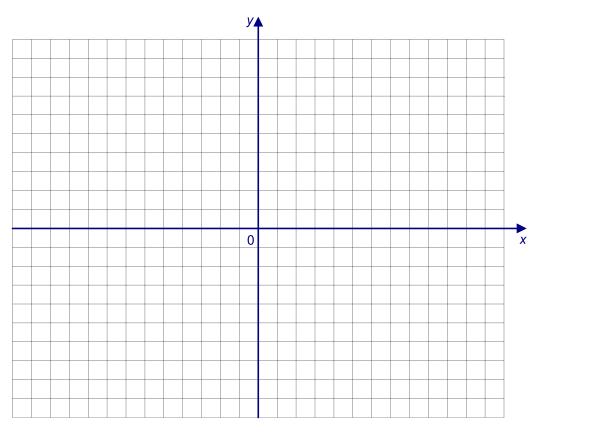
\includegraphics[ width=4.8663in, height=3.4956in,]{L4SZ2705}
	}
	\begin{enumerate}
		\item Show the points $A \left (3 ,5\right )$ and $B \left ( -2 , -5\right )$ on the graph. 
		
		\item Calculate the slope of the line through $A$ and $B$. i.e. the slope of $\bar{AB}\text{.}$ 
		
		\item What is the equation of the line $A B$? 
		
		\item What is the equation of the line parallel to the line $A B$ through the point $\left ( -2 ,3\right )\text{?}$ 
		
		\item Starting from the point $B$ on the graph frame draw a line with a slope of $\frac{4}{5}\text{.}$ 
	\end{enumerate}

  	
	\item 
	If $f (x) =x^{2}$ and $g (x) =x^{3}$ evaluate 
	
	
	\begin{enumerate}
		\item $f (2)$ 
		
		\item $f ( -2)$ 
		
		\item $g (3)$ 
		
		\item $g ( -3)\vspace{+5.000000cm}$ \end{enumerate}
	
	
	\item 
	Complete the table of values for the function $g (x) =x^{3} -x$ and sketch the graph\vspace{0.5cm} \\\relax
	\begin{tabular}[c]{cc}\hline
		$x$  & $g (x) =x^{3} -x$  \\
		\hline
		$ -1.5\rule[-8pt]{0pt}{24pt}$  & \ \ \ \ \ \ \ \ \ \ \ \ \ \ \ \ \ \ \  \\
		\hline
		$ -1\rule[-8pt]{0pt}{24pt}$  &  \\
		\hline
		$ -0.5\rule[-8pt]{0pt}{24pt}$  &  \\
		\hline
		$0\rule[-8pt]{0pt}{24pt}$  &  \\
		\hline
		$0.5\rule[-8pt]{0pt}{24pt}$  &  \\
		\hline
		$1\rule[-8pt]{0pt}{24pt}$  &  \\
		\hline
		$1.5\rule[-8pt]{0pt}{24pt}$  &  \\
		\hline
	\end{tabular} \\\relax
	\setlength\fboxrule{0in}\setlength\fboxsep{0.2in}\fcolorbox[HTML]{000000}{FFFFFF}{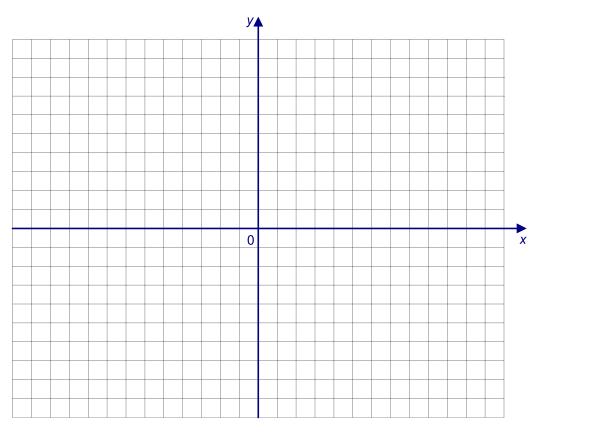
\includegraphics[ width=4.8663in, height=3.4956in,]{L4SZ2706}
	}
	 
	
	\item  Given $f (x) =\left (x +3)(x -1\right )\left (x +1\right )^{2}$ 
	

	\begin{enumerate}
		\item What is the degree of the polynomial? 
		
		\item Where does
		the graph cut the $x$-axis? (I.e. what are the zeros?) 
		
		\item Where does the graph cut the $y$-axis? 
		
		\item Sketch the graph \\\relax
		\setlength\fboxrule{0in}\setlength\fboxsep{0.2in}\fcolorbox[HTML]{000000}{FFFFFF}{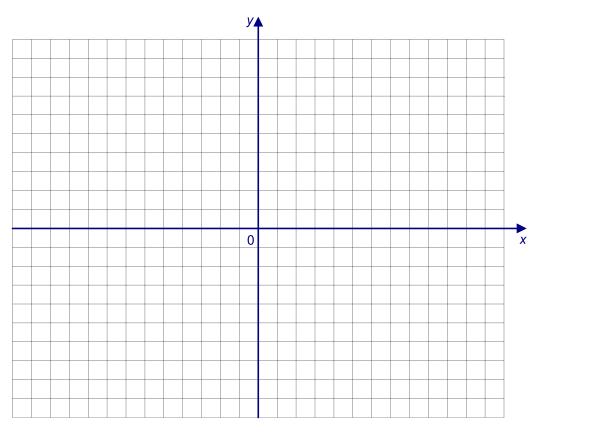
\includegraphics[ width=4.561in, height=3.2759in,]{L4SZ2707}
		}
	\end{enumerate}

	\item Fill in the
	table and draw the graph of $y =\genfrac{(}{)}{}{}{1}{2}^{x}\vspace{+0.500000cm}$ \\\relax
	\begin{tabular}[c]{|c|c|c|c|c|c|c|c|}\hline
		$x$  & -3  & -2  & -1
		& 0  & 1  & 2  & 3
		\\
		\hline
		$y =\genfrac{(}{)}{}{}{1}{2}^{x}$  & \ \ \ \ \ \rule[-8pt]{0pt}{24pt}
		& \ \ \ \ \ \rule[-8pt]{0pt}{24pt}
		& \ \ \ \ \ \rule[-8pt]{0pt}{24pt}
		& \ \ \ \ \ \rule[-8pt]{0pt}{24pt}
		& \ \ \ \ \ \rule[-8pt]{0pt}{24pt}
		& \ \ \ \ \ \rule[-8pt]{0pt}{24pt}
		& \ \ \ \ \ \rule[-8pt]{0pt}{24pt}
		\\
		\hline
	\end{tabular} \\\relax
	\setlength\fboxrule{0in}\setlength\fboxsep{0.2in}\fcolorbox[HTML]{000000}{FFFFFF}{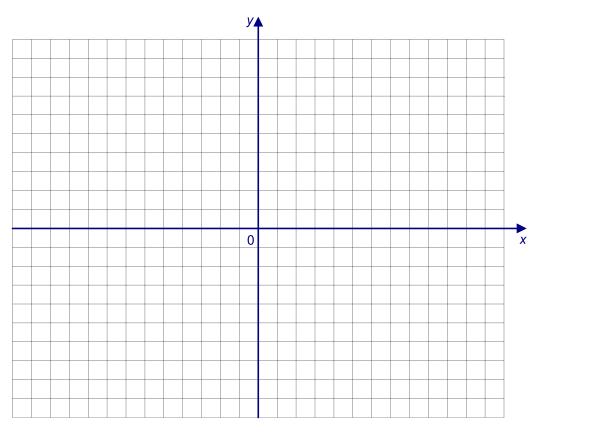
\includegraphics[ width=4.4771in, height=3.2162in,]{L4SZ2708}
	}
	
	
	
	\begin{enumerate}
		\item [(b)] Evaluate 
		
		
		\begin{enumerate}
			\item $3^{3.4}$ 
			
			\item $e^{ -0.6}$ \end{enumerate}
	\end{enumerate}
	
	
	\item 
	Write the equivalent logarithm statement. One is done for you. 
	
	
	\begin{enumerate}
		\item
		\begin{enumerate}
			\item $64 =2^{6} \Leftrightarrow \log _{2} 64 =6$ 
			
			\item $0.01 =10^{ -2} \Leftrightarrow $ \end{enumerate}
		
		
		\item [(b)]
		Write the equivalent statement using an exponent. 
		
		
		\begin{enumerate}
			\item $\log _{5} 625 =4 \Leftrightarrow $ 
			
			\item $\log _{a} k =t \Leftrightarrow $ \end{enumerate}
		
		
		\item [(c)]
		Calculate the value for 
		
		
		\begin{enumerate}
			\item $\log _{9} 9$ 
			
			\item $\log _{2} \genfrac{(}{)}{}{}{1}{8}$ 
			
			\item $\log  1000$ 
			
			\item $\ln  2.95$ 
			
			\item $\ln  e^{3.1}$ 
			
			\item $\log _{4} 0.25$ \end{enumerate}
	\end{enumerate}

	\item Write the following as the logarithm of a single number 
	
	
	\begin{enumerate}
		\item $\log _{4} 7 +\log _{4} 5$ 
		
		\item $\log _{5} 18 -\log _{5} 3$ 
		
		\item $2 \log _{3} 4$ 
		
		\item $\log _{4} 5 +\log _{4} 2 -\log _{4} 10 +3 \log _{4} 2$ \end{enumerate}	
\end{enumerate}

\section*{Some Answers}
\begin{tabular}[c]{rrlr}1.  & (a)
	& $ -x -y$  &  \\
	& (b)
	& $ -15 x +6 y$  &  \\
	&  &  &  \\
	2.
	&  & $2\frac{1}{2}$  &  \\
	&  &  &  \\
	3.
	& (a)  & $1$  &  \\
	& (b)
	& $0.01$  &  \\
	&  &  &  \\
	4.
	& (a)  & $9 a^{4} b^{2}$  &  \\
	& (b)
	& $\frac{x^{6}}{27}$  &  \\
	&  &  &  \\
	5.
	&  & $1.28$  &  \\
	&  &  &  \\
	6.
	& (a)  & $x^{2} +3 x +2$  &  \\
	& (b)
	& $4 x^{2} -1$  &  \\
	&  &  &  \\
	7.
	& (a)  & $\left (x +7\right ) \left (x +4\right )$  &  \\
	& (b)
	& $\left (2 x +3\right ) \left (x -4\right )$  &  \\
	&  &  &  \\
	8.
	&  & $\frac{x +2}{x -1}$  &  \\
	&  &  &  \\
	9.
	& (a)  & $3.16$  &  \\
	& (b)
	& $ -1.87$ or $5.87$  &  \\
	&  &  &  \\
	10.
	& (a)  & $4$ or $ -2$  &  \\
	& (b)
	& $0.637$ or $ -3.137$  &  \\
	&  &  &  \\
	11.
	& (a)  & $t =\frac{v -u}{a}$  &  \\
	& (b)
	& $t =\frac{1}{\alpha } \left (\frac{l}{l_{0}} -1\right )$  &  \\
	&  &  &  \\
	12.
	&  & $79.4 \mathrm{m}^{3}$  &  \\
	&  &  &  \\
	13.
	&  & Parabola with vertex $\left (0 , -3\right )$  & 
\end{tabular}

\relax    
\setlength\fboxrule{0.01in}\setlength\fboxsep{0.2in}\fcolorbox[HTML]{000000}{FFFFFF}{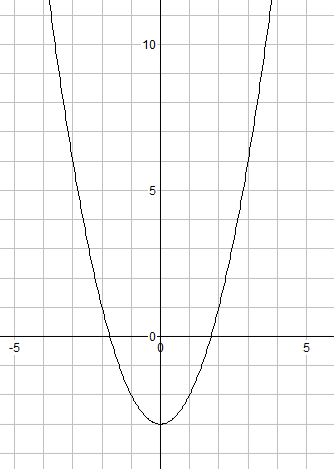
\includegraphics[ width=2.0496in, height=2.8669in,]{L4SZ2709}
}
\\ 
\\



\begin{tabular}[c]{rrlr}14.  &  & $3.61$  &  \\
	&  &  &  \\
	15.
	&  & x-intercepts $1.73$ and $ -1.73$  &  \\
	&  & y-intercept
	$ -3$  &  \\
	&  &  &  \\
	16.
	& (a)  & On the graph below  &  \\
	& (b)
	& $2$  &  \\
	& (c)
	& $y =2 x -1$  &  \\
	& (d)
	& $y =2 x +7$  & 
\end{tabular}

16. (e)
\setlength\fboxrule{0.01in}\setlength\fboxsep{0.2in}\fcolorbox[HTML]{000000}{FFFFFF}{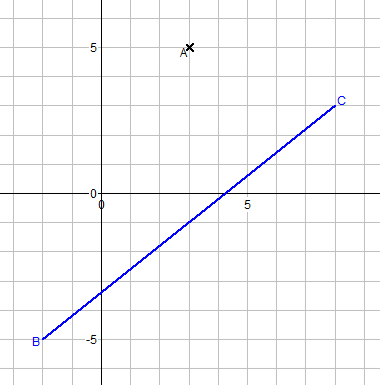
\includegraphics[ width=2.8297in, height=2.8669in,]{L4SZ270A}
}
\\ 
\\



\begin{tabular}[c]{rrrr}17.  & (a)
	& $4$  &  \\
	& (b)
	& $4$  &  \\
	& (c)
	& $27$  &  \\
	& (d)
	& $ -27$  & 
\end{tabular}

18.
\begin{tabular}[c]{|c|c|}\hline
	$x$  & $g (x) =x^{3} -x$  \\
	\hline
	$ -1.5$  & $ -1.875\;$  \\
	\hline
	$ -1$  & $0$  \\
	\hline
	$ -0.5$  & $0.375$  \\
	\hline
	$0$  & $0$  \\
	\hline
	$0.5$  & $ -0.375$  \\
	\hline
	$1$  & $0$  \\
	\hline
	$1.5$  & $1.875$  \\
	\hline
\end{tabular}\vspace{0.5cm} \\\relax
\setlength\fboxrule{0.01in}\setlength\fboxsep{0.2in}\fcolorbox[HTML]{000000}{FFFFFF}{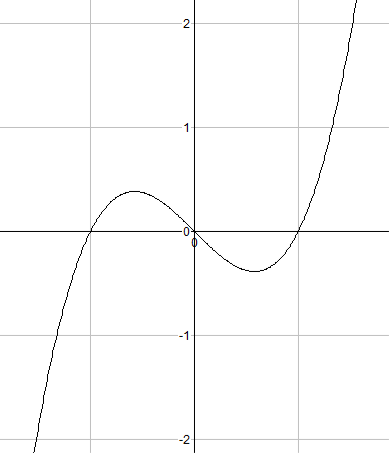
\includegraphics[ width=2.4656in, height=2.866in,]{L4SZ270B}
}


$
\begin{tabular}[c]{rrlr}19. 
& (a)
& $4$
& 
\\
& (b)
& $ -3$, $1$, $ -1$ (touches) 
& 
\\
& (c)
& $ -3$
& 
\end{tabular}\vspace{+0.500000cm}$ 

19.(d)    
\setlength\fboxrule{0.01in}\setlength\fboxsep{0.2in}\fcolorbox[HTML]{000000}{FFFFFF}{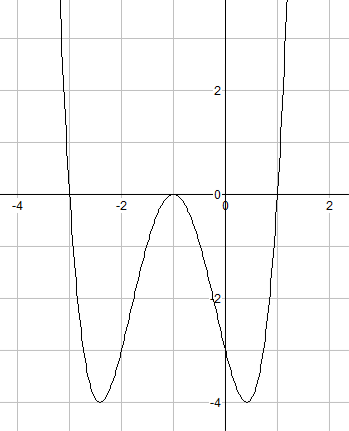
\includegraphics[ width=2.3263in, height=2.866in,]{L4SZ270C}
}


20. (a) $8 ,4 ,2 ,1 ,\frac{1}{2} ,\frac{1}{4} ,\frac{1}{8}\vspace{+0.500000cm}$ \\\relax    
\setlength\fboxrule{0.01in}\setlength\fboxsep{0.2in}\fcolorbox[HTML]{000000}{FFFFFF}{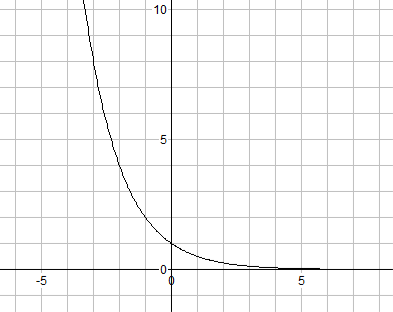
\includegraphics[ width=3.1782in, height=2.5278in,]{L4SZ270D}
}



\begin{tabular}[c]{rrrl}20.  & (b)
	& 1.  & $41.9$  \\
	&  & 2.
	& $0.5488$  \\
	&  &  &  \\
	21.
	& (a)  &  & $\log _{10} 0.01 = -2$  \\
	& (b)  & 1.
	& $625 =5^{4}$  \\
	&  & 2.
	& $k =a^{t}$  \\
	& (c)  & 1.
	& $1$  \\
	&  & 2.
	& $ -3$  \\
	&  & 3.
	& $3$  \\
	&  & 4.
	& $1.082$  \\
	&  & 5.
	& $3.1$  \\
	&  & 6.
	& $ -1$  \\
	&  &  &  \\
	22.
	& (a)  &  & $\log _{4} 35$  \\
	& (b)  &  & $\log _{5} 6$  \\
	& (c)  &  & $\log _{3} 16$  \\
	& (d)  &  & $\log _{4} 8$  \\
	&  &  &  \\

\end{tabular} 
\clearpage
\section*{Factoring Exercises}
Some exercises look quite difficult on the surface but quickly look like a
familiar one once you get started. 

\subsubsection{Example}
Completely factor the following expression: $x^{4} +2 x^{3} -3 x^{2}$\\
Start by removing the common factor to all terms: $x^2$\\
\begin{eqnarray*} x^{4} +2 x^{3} -3 x^{2} &= x^{2} \left (x^{2} +2 x -3\right ) \\
	\text{then factor the remaining term as usual}\\
	 &= x^{2} \left (x -1\right ) \left (x +3\right )\end{eqnarray*}


Solve the following equations both algebraically and graphically.
*Note there are no answers for these exercises. Want to make some? Email them to Jeff!
\begin{enumerate}
	\item   
	\columnsep =30pt
	\begin {multicols}{2}
	$x -4 =5 x +12$ 
	
	\item $\frac{1}{2} x -3 =6 +2 x$ 
	
	\item $\frac{2}{x} +\frac{1}{2 x} =7$ 
	
	\item $\frac{4}{x +2} -\frac{6}{2 x} =\frac{5}{2 x +4}$ 
	
	\item $x^{2} -32 =0$ 
	
	\item $x^{3} +16 =0$ 
	
	\item $16 x^{4} =625$ 
	
	\item $2 x^{5} -243 =0$ 
	
	\item $\left (x -5\right )^{4} -80 =0$ 
	
	\item $6 \left (x +2\right )^{5} =64$ 
	\end {multicols}

\end{enumerate}


Find all real solutions of these equations correct to two decimal places (d.p.). 


\begin{enumerate}
	  
	\columnsep =30pt
	\begin {multicols}{2}\setcounter{enumi}{10}\item
	$x^{3} -2 x^{2} -x -1 =0$ 
	
	\item $x^{4} -8 x^{2} +2 =0$ 
	
	\item $x \left (x -1\right ) \left (x +2\right ) =\frac{1}{6} x$ 
	
	\item $x^{4} =16 -x^{3}$ 
	\end {multicols}

\end{enumerate}


Solve these inequalities correct to two d.p. 
\begin{enumerate}
	\setcounter{enumi}{14}\item   
	\columnsep =30pt
	\begin {multicols}{2}
	$x^{2} -3 x -10 \leq 0$ 
	
	\item $0.5 x^{2} +0.875 x \leq 0.25$ 
	
	\item  $x^{3} +11 x \leq 6 x^{2} +6$ 
	
	\item $16 x^{3} +24 x^{2} > -9 x -1$ 
	
	\item  $x^{\frac{1}{3}} <x$ 
	
	\item  $\left (x +1\right )^{2} <\left (x -1\right )^{2}$ 
	\end {multicols}

\end{enumerate}

\section{Systems Exercises}
Solve the following linear systems of two equations with two unknowns using an appropriate method.
\begin{description}
	\columnsep =30pt
	\begin {multicols}{2}
	\item [a.]   	
	$\left \{
	\begin{tabular}[c]{rrr}$x +y$
	& $ =$
	& $4$
	\\
	$2 x -y$
	& $ =$
	& $2$
	\end{tabular}\right .$ \\
	
	\item [b.]
	$\left \{
	\begin{tabular}[c]{rrr}$2 x +y$
	& $ =$
	& $11$
	\\
	$x -2 y$
	& $ =$
	& $4$
	\end{tabular}\right .$ \\
	
	
	\item [c.]   	
	$\left \{
	\begin{tabular}[c]{rrr}$2 x -3 y$
	& $ =$
	& $12$
	\\
	$ -x +\frac{3}{2} y$
	& $ =$
	& $4$
	\end{tabular}\right .$ \\
	
	\item [d.]
	$\left \{
	\begin{tabular}[c]{rrr}$2 x +6 y$
	& $ =$
	& $0$
	\\
	$ -3 x -9 y$
	& $ =$
	& $18$
	\end{tabular}\right .$ \\
	
	\item [e.]   
	$\left \{
	\begin{tabular}[c]{rrr}$ -x +\frac{1}{2} y$
	& $ =$
	& $ -5$
	\\
	$2 x -y$
	& $ =$
	& $10$
	\end{tabular}\right .$ \\
	
	\item [f.]
	$\left \{
	\begin{tabular}[c]{rrr}$12 x +15 y$
	& $ =$
	& $ -18$
	\\
	$2 x + 5 y$
	& $ =$
	& $ -3$
	\end{tabular}\right .$ \\
	\end {multicols}
	
\end{description}

Use the substitution method to find all solutions of the system of equations. *Note that some are non-linear equations.

\begin{description}
	
	\columnsep =30pt
	\begin {multicols}{2}
	\item [1.]   
	$\left \{
	\begin{tabular}[c]{rrr}$x -y$
	& $ =$
	& $2$
	\\
	$2 x +3 y$
	& $ =$
	& $9$
	\end{tabular}\right .$ 
	
	\item [3.]
	$\left \{
	\begin{tabular}[c]{lll}$y$
	& $ =$
	& $x^{2}$
	\\
	$y$
	& $ =$
	& $x +12$
	\end{tabular}\right .$ 
	\end {multicols}
	
	
	\item [5.]   
	\columnsep =30pt
	\begin {multicols}{2}
	%EndExpansion
	$\left \{
	\begin{tabular}[c]{rrr}$x^{2} +y^{2}$
	& $ =$
	& $8$
	\\
	$x +y$
	& $ =$
	& $0$
	\end{tabular}\right .$ 
	
	\item [7.]
	$\left \{
	\begin{tabular}[c]{rrr}$x +y^{2}$
	& $ =$
	& $0$
	\\
	$2 x +5 y^{2}$
	& $ =$
	& $75$
	\end{tabular}\right .$ 
	\end {multicols}
	
\end{description}

Use the elimination method to find
all solutions of the system of equations 


\begin{description}
	\item [9.]   
	%TCIMACRO{\TeXButton{Start Two Columns}{\columnsep =30pt
	% \begin {multicols}{2}}}%
	%BeginExpansion
	\columnsep =30pt
	\begin {multicols}{2}
	%EndExpansion
	$\left \{
	\begin{tabular}[c]{rrr}$x +2 y$
	& $ =$
	& $5$
	\\
	$2 x +3 y$
	& $ =$
	& $8$
	\end{tabular}\right .$ 
	
	\item [11.]
	$\left \{
	\begin{tabular}[c]{rrr}$x^{2} -2 y$
	& $ =$
	& $1$
	\\
	$x^{2} +5 y$
	& $ =$
	& $29$
	\end{tabular}\right .$ 
	%TCIMACRO{\TeXButton{End Two Columns}{\end {multicols}}}%
	%BeginExpansion
	\end {multicols}
	%EndExpansion
	
	
	\item [13.] $\left \{
	\begin{tabular}[c]{rrr}$3 x^{2} -y^{2}$
	& $ =$
	& $11$
	\\
	$x^{2} +4 y^{2}$
	& $ =$
	& $8$
	\end{tabular}\right .$ \end{description}

Find all solutions of the system of equations 


\begin{description}
	\item [17.]   
	%TCIMACRO{\TeXButton{Start Two Columns}{\columnsep =30pt
	% \begin {multicols}{2}}}%
	%BeginExpansion
	\columnsep =30pt
	\begin {multicols}{2}
	%EndExpansion
	$\left \{
	\begin{tabular}[c]{rrr}$y +x^{2}$
	& $ =$
	& $4 x$
	\\
	$y +4 x$
	& $ =$
	& $16$
	\end{tabular}\right .$ 
	
	\item [18.]
	$\left \{
	\begin{tabular}[c]{rrr}$x -y^{2}$
	& $ =$
	& $0$
	\\
	$y -x^{2}$
	& $ =$
	& $0$
	\end{tabular}\right .$ 
	%TCIMACRO{\TeXButton{End Two Columns}{\end {multicols}}}%
	%BeginExpansion
	\end {multicols}
	%EndExpansion
	
	
	\item [21.]   
	%TCIMACRO{\TeXButton{Start Two Columns}{\columnsep =30pt
	% \begin {multicols}{2}}}%
	%BeginExpansion
	\columnsep =30pt
	\begin {multicols}{2}
	%EndExpansion
	$\left \{
	\begin{tabular}[c]{rrr}$x -y$
	& $ =$
	& $4$
	\\
	$x y$
	& $ =$
	& $12$
	\end{tabular}\right .$ 
	
	\item [25.]
	$\left \{
	\begin{tabular}[c]{rrr}$x^{2} +y^{2}$
	& $ =$
	& $9$
	\\
	$x^{2} -y^{2}$
	& $ =$
	& $1$
	\end{tabular}\right .$ 
	%TCIMACRO{\TeXButton{End Two Columns}{\end {multicols}}}%
	%BeginExpansion
	\end {multicols}
	%EndExpansion
\end{description}

Use a graphical method to find all solutions of the system of equations correct
to 2 decimal places 


\begin{description}
	\item [31.]   
	%TCIMACRO{\TeXButton{Start Two Columns}{\columnsep =30pt
	% \begin {multicols}{2}}}%
	%BeginExpansion
	\columnsep =30pt
	\begin {multicols}{2}
	%EndExpansion
	$\left \{
	\begin{tabular}[c]{rrr}$y$
	& $ =$
	& $2 x +6$
	\\
	$y$
	& $ =$
	& $ -x +5$
	\end{tabular}\right .$ 
	
	\item [35.]
	$\left \{
	\begin{tabular}[c]{rrr}$x^{2} +y^{2}$
	& $ =$
	& $25$
	\\
	$x +3 y$
	& $ =$
	& $2$
	\end{tabular}\right .$ 
	%TCIMACRO{\TeXButton{End Two Columns}{\end {multicols}}}%
	%BeginExpansion
	\end {multicols}
	%EndExpansion
	
	
	\item [37.] $\left \{
	\begin{tabular}[c]{lrr}$\frac{x^{2}}{9} +\frac{y^{2}}{18} =1$
	& 
	& 
	\\
	$y = -x^{2} +6 x -2$
	& 
	& 
	\end{tabular}\right .$ \end{description}

Word problems 


\begin{description}
	\item [41.] A rectangle has an area of $180 cm^{2}$ and a perimeter of $54 \mbox{cm}$. What are its dimensions? 
	
	\item [42.]
	A right-angled triangle has an area of $84 cm^{2}$ and a hypotenuse $25 \mbox{cm}$ long. What are the lengths of the other two sides?
	
	
	\item [44.] A circular piece of sheet metal has a diameter
	of $20 \mbox{cm}$. the edges are to be cut off to form a rectangle
	of area $160 cm^{2}$. What are the dimensions of the rectangle? 
	
	\item \qquad \qquad \qquad \qquad \qquad \qquad
	\setlength\fboxrule{0in}\setlength\fboxsep{0.2in}\fcolorbox[HTML]{000000}{FFFFFF}{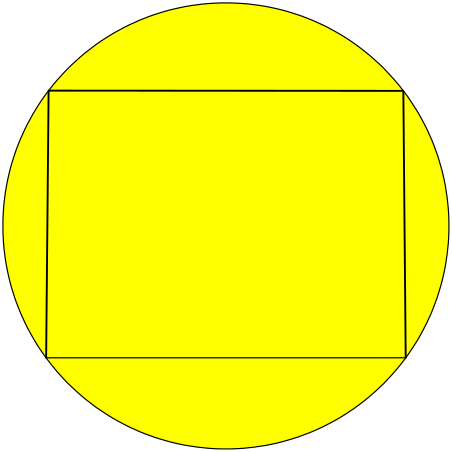
\includegraphics[ width=2.6385in, height=2.6385in,]{L4SZ270E}
	}
	
	
	\item [46.] A rectangular piece of sheet metal with and
	area of $1200 cm^{2}$ is to be bent into a cylindrical length of pipe having a volume of $600 cm^{3}$. What are the dimensions of the sheet of metal? \end{description}

\begin{description}
	\item [47.] The admission fee at an amusement park is $ \$1.50$ for children and $ \$4.00$ for adults. On a certain day, $2200$ people entered the park and the admission fees collected totalled $ \$5050$. How many children and how many adults were admitted? 
	
	\item [48.]
	A man flies a small aeroplane from Fargo to Bismarck, North Dakota - a distance of $180 \mbox{mi}$. Because he is flying into a headwind, the trip
	takes him $2$ hours. On the way back, the wind is still blowing at the same speed, so the return
	trip takes only $1$ hour and $12$ minutes. What is his speed in still air and how fast is the wind blowing? 
	
	\item [49.]
	A woman keeps fit by bicycling and running every day. One Monday she spends $\frac{1}{2} \mbox{h}$ at each activity and covers a total of $12\frac{1}{2} \mbox{mi}$. On Tuesday she runs for $12 \mbox{min}$ and cycles for $45 \mbox{min}$, covering a total of $16 \mbox{mi}$. Assuming her running and cycling speeds don't
	change from day to day, find these speeds. 
	
	\item [50.] A customer
	in a coffee shop purchases a blend of two coffees: Kenyan, costing $ \$3.50$ a pound, and Sri Lankan, costing $ \$5.60$ a pound. He buys $3 \mbox{lb}$ of the blend, which costs him $ \$11.55$. How many pounds of each kind went into the mixture?
\end{description}


\section{Some Answers}

\columnsep =30pt
\begin {multicols}{2}

\textbf{Linear Only:}

a. $\left (2 ,2\right )$ 

b. $\left (5.2 ,0.6\right )$

c. no solutions

d. no solutions

e. infinite solutions

f. $\left (-1.5 ,0\right )$\\
\break
\textbf{Mixed:}

1. $\left (3 ,1\right )$ 

3. $\left (4 ,16\right )$ 

5. $\left (2 , -2\right ) ,\left ( -2 ,2\right )$ 

7. $\left ( -25 ,5\right ) ,\left ( -25 , -5\right )$ 

9. $\left (1 ,2\right )$ 

11. $\left ( -3 ,4\right ) ,\left (3 ,4\right )$ 

13. $\left ( -2 , -1\right ) ,\left ( -2 ,1\right ) ,\left (2 , -1\right ) ,\left (2 ,1\right )$ 

17. $\left (4 ,0\right )$ 

18. $\left (0 ,0\right ) ,\left (1 ,1\right )$ 

21. $\left (6 ,2\right ) ,\left ( -2 , -6\right )$ 

25. $\left (\sqrt{5} ,2\right )\left (\sqrt{5} , -2\right )$ 

31. $\left ( -0.33 ,5.33\right )$ 

35. $\left ( -4.51 ,2.17\right ) ,\left (4.91 , -0.97\right )$ 

37. $\left (1.23 ,3.87\right ) ,\left ( -0.35 , -4.21\right )$ \\
\break
\textbf{Word Problems}\\

41. $12 \mbox{cm}$ by $15 \mbox{cm}$ 

42. $7 \mbox{ft}$ and $24 \mbox{ft}$ 

44. $4 \sqrt{5} \mbox{in}$ by $8 \sqrt{5} \mbox{in}$ 

46. The dimensions of the sheet are $2 \pi $ by $\frac{600}{\pi }$  

47. The number of children admitted was 1500 and the number
of adults was 700. 

48. Plane's speed $120 mi/\mbox{h}$, wind speed $30 mi/\mbox{h}$ 

49. Run $5 mi/\mbox{h}$, cycle $20 mi/\mbox{h}$ 

50. $2.5$ pounds of Kenyan coffee and $0.5$ pounds of Sri Lankan coffee should be mixed. 

\end {multicols}

